\documentclass[tikz,border=5pt]{standalone}
\usepackage{tikz}
\usetikzlibrary{decorations.pathreplacing} % Required for the brace

% --- Define Colors for the Schematic ---
\definecolor{fieldGreen}{HTML}{2E8B57} % SeaGreen
\definecolor{lineWhite}{HTML}{ECF0F1}  % Off-white for lines
\definecolor{teamRed}{HTML}{E74C3C}    % A nice flat red
\definecolor{teamBlue}{HTML}{3498DB}   % A nice flat blue
\definecolor{rodGray}{HTML}{95A5A6}    % Metal rod color
\definecolor{tableWood}{HTML}{7E5109}  % Brown frame border

\begin{document}

% Adjust scale=... to fit your slide.
% scale=0.6 usually works well within a standard Beamer frame column.
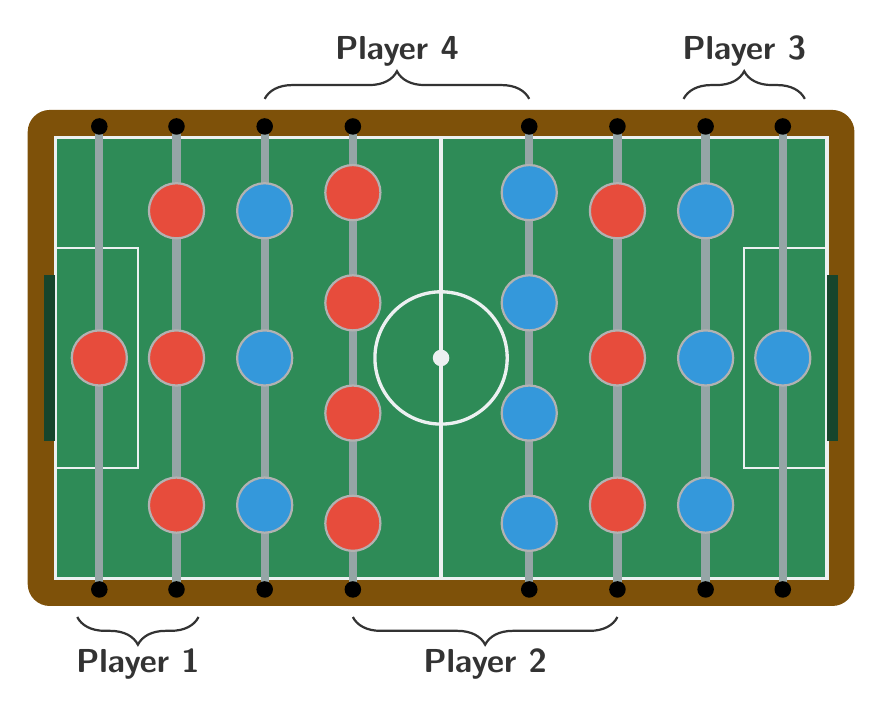
\begin{tikzpicture}[scale=0.7, >=stealth]

    % --- 1. The Table and Field ---
    % Outer Wood Frame
    \fill[tableWood, rounded corners=8pt] (-7.5, -4.5) rectangle (7.5, 4.5);
    
    % The Green Playing Field
    \fill[fieldGreen] (-7, -4) rectangle (7, 4);
    
    % Field Border Lines
    \draw[lineWhite, very thick] (-7, -4) rectangle (7, 4);


    % --- 2. Field Markings ---
    % Center Line
    \draw[lineWhite, very thick] (0, -4) -- (0, 4);
    
    % Center Circle
    \draw[lineWhite, very thick] (0,0) circle (1.2cm);
    \fill[lineWhite] (0,0) circle (0.15cm); % Center dot
    
    % Goal Areas (Crease)
    \draw[lineWhite, thick] (-7, -2) rectangle (-5.5, 2);
    \draw[lineWhite, thick] (7, -2) rectangle (5.5, 2);

    % The Goals (Visual openings at the ends)
    \fill[fieldGreen!50!black] (-7.2, -1.5) rectangle (-7, 1.5);
    \fill[fieldGreen!50!black] (7, -1.5) rectangle (7.2, 1.5);


    % --- 3. The Rods ---
    % We define the x-positions for standard 1-2-5-3 setup
    % R=Red side, B=Blue side
    % Goalie, Defenders, Midfield, Strikers
    \foreach \x in {-6.2, -4.8, -3.2, -1.6,  1.6, 3.2, 4.8, 6.2} {
        \draw[rodGray, line width=3pt, line cap=round] (\x, -4.2) -- (\x, 4.2);
        % Add little rubber bumpers on ends of rods
        \fill[black] (\x, -4.2) circle (0.15);
        \fill[black] (\x, 4.2) circle (0.15);
    }


    % --- 4. The Players ---
    % Define common player style
    \tikzstyle{player}=[circle, draw=black!30, thick, minimum size=0.7cm, inner sep=0pt, outer sep=0pt]

    % --- RED TEAM (Left Side) ---
    
    % Goalie (1 player)
    \node[player, fill=teamRed] at (-6.2, 0) {};
    
    % Defenders (3 players)
    \foreach \y in {-2.67, 0, 2.67}
        \node[player, fill=teamRed] at (-4.8, \y) {};
        
    % Midfield (4 players) - Red team's midfield is usually on the "away" side
    \foreach \y in {-3, -1, 1, 3}
        \node[player, fill=teamRed] at (-1.6, \y) {};

    % Strikers (3 players)
    \foreach \y in {-2.67, 0, 2.67}
        \node[player, fill=teamRed] at (3.2, \y) {};

    % Player label
    \draw[decorate, decoration={brace, amplitude=10pt, mirror}, thick, black!80] 
        (-6.6, -4.7) -- (-4.4, -4.7) 
        node[midway, yshift=-0.6cm, font=\sffamily\bfseries\large] {Player 1};
    
    \draw[decorate, decoration={brace, amplitude=10pt, mirror}, thick, black!80] 
         (-1.6, -4.7) -- (3.2, -4.7) 
         node[midway, yshift=-0.6cm, font=\sffamily\bfseries\large] {Player 2};


    % --- BLUE TEAM (Right Side) ---
    
    % Goalie (1 player)
    \node[player, fill=teamBlue] at (6.2, 0) {};
    
    % Defenders (3 players)
    \foreach \y in {-2.67, 0, 2.67}
        \node[player, fill=teamBlue] at (4.8, \y) {};
        
    % Midfield (4 players) - Blue team's midfield
    \foreach \y in {-3, -1, 1, 3}
        \node[player, fill=teamBlue] at (1.6, \y) {};

    % Strikers (3 players)
    \foreach \y in {-2.67, 0, 2.67}
        \node[player, fill=teamBlue] at (-3.2, \y) {};
    
    % Player label
    \draw[decorate, decoration={brace, amplitude=10pt, mirror}, thick, black!80] 
        (6.6, 4.7) -- (4.4, 4.7) 
        node[midway, yshift=0.6cm, font=\sffamily\bfseries\large] {Player 3};
    
    \draw[decorate, decoration={brace, amplitude=10pt, mirror}, thick, black!80] 
         (1.6, 4.7) -- (-3.2, 4.7) 
         node[midway, yshift=0.6cm, font=\sffamily\bfseries\large] {Player 4};

    % --- 5. Optional Labels ---
    %\node[text=red, font=\sffamily\bfseries] at (-6, 4.8) {RED GOAL};
    %\node[text=blue, font=\sffamily\bfseries] at (6, 4.8) {BLUE GOAL};
    
\end{tikzpicture}
\end{document}